 \documentclass[rgb, pdf]{beamer}
\usepackage{listings}
\usepackage[algoruled,boxed,vlined]{algorithm2e}
\makeatletter 
\g@addto@macro{\@algocf@init}{\SetKwInOut{Parameters}{Parameters}} 
\makeatother
\newcommand{\hrulealg}[0]{\vspace{1mm} \hrule \vspace{1mm}}


\usetheme{Konstanz}
\format{169}

\title{Minimization of Weighted Automata}
\titleCorporateDesign{Minimization}{of}{Weighted}{Automata}
\author{Fabian Klopfer}
\date{12.06.2020}
\institute{Modelling of Complex Self-Organizing Systems Group}

\bibliography{resources}
%\renewcommand*{\bibfont}{\tiny}

\begin{document}
    \usebeamerfont{normalfont}
    \begin{frame}
        \titlepage
    \end{frame}

    \begin{frame}{Introduction}
        In the last presentation $\dots$ \\ \vspace{0.5cm}
        \begin{itemize}
            \item two models for stochastic dynamical systems were considered: \\ \vspace{0.2cm} 
                Weighted Automata (WA) and Differential Equations (DE)\\ \vspace{0.8cm} 
            \item an example for modelling a CRN's dynamics in both models was given: \\
            \vspace{0.3cm} 
            \begin{itemize}
             \item[DE] Solving Chemical Master Equation 
             \item[WA] Monte Carlo CTMC
            \end{itemize}
        \end{itemize}
    \end{frame}
    \begin{frame}{Goals specified}
        \begin{enumerate}
            \item Implement minimization algorithm for weighted automata \autocite{Kiefer2013OnTC}. {\Huge $\checkmark$ }  \\ \vspace{0.7cm}
            \item Implement model reduction algorithm for ODEs \autocite{Cardelli2017MaximalAO}.  \\ \vspace{0.7cm}
            \item Develop reproducible benchmarks  \\ \vspace{0.7cm}
            \item Write report \\
        \end{enumerate}
    \end{frame}
    
    \begin{frame}{What has been done so far}
        \begin{itemize}
            \item Software Requirement Specification \& Software Design Document \\ \vspace{0.7cm}
            \item Random Basis Minimal WA Construction Algorithm by Kiefer/Schützenberger~\autocite{Kiefer2013OnTC} \\ \vspace{0.7cm}
            \item Execution of example by Matlab script and hand \\ \vspace{0.7cm}
            \item Implementation of minimization \& equivalence algorithm, interfaces, TUI, CLI, tests \\ \vspace{0.7cm}
        \end{itemize}
    \end{frame}
    
    \begin{frame}[allowframebreaks]{The Weighted Automaton Minimization Algorithm~\autocite{Kiefer2013OnTC}}
        Weighted Automaton $A = \left( n, \Sigma, \alpha, \mu, \eta \right)$, where
        \begin{itemize}
         \item $n$ the number of states
         \item $\Sigma$ the input alphabet
         \item $\alpha$ the initial vector with a non-zero value for all starting states
         \item $\mu$ the set of transition matrices, one per input character
         \item $\eta$ the final vector with non-zero values for all ending states
        \end{itemize}
        \vspace{7cm}
        Reduction to Schwarz-Zippel Lemma (Polynomial Identity Testing) provide bounds on correctness $\frac{n}{K}$\\ \vspace{0.5cm}
        Author claims complexity is in $\mathcal{NC}$, this is not correct (c.f. later) \\ \vspace{0.5cm}
        In the following slides use forward reduction, the backwards reduction is similar
        \framebreak
        
        \begin{itemize}
         \item Find a basis $F$ of the prefix space using random vectors $r_i$
         \begin{itemize}
          \item Add the vectors of all prefix words up to length n together and multiply this vector by n different factors yielding $\{v_1, \dots, v_n\}$
          \item Factors are derived by random vectors and structure of prefixes
          \item Base is then the maximally linear independent subset of $\{ \alpha, v_1, \dots, v_n\}$
         \end{itemize}
         \vspace{0.5cm}
         \item Use basis to do Schützenberger Construction~\autocite{schutz}: $\overrightarrow{A} = (\overrightarrow{n}, \Sigma, \overrightarrow{\alpha}, \overrightarrow{\mu}, \overrightarrow{\eta})$
            With
            \begin{itemize}
             \item $\overrightarrow{\mu} = \overrightarrow{F} \mu \overrightarrow{F}^{-1}$ or $\overrightarrow{F} \mu = \overrightarrow{\mu} \overrightarrow{F}$
             \item $\overrightarrow{\alpha} = e_1$
             \item $\overrightarrow{\eta} = \overrightarrow{F}\eta$
             \item $\overrightarrow{n} = \text{rank}(\overrightarrow{\mu})$
            \end{itemize}

        \end{itemize}
    \end{frame}

    \begingroup
    \large
    \begin{frame}[allowframebreaks]{The Weighted Automaton Minimization Algorithm: Pseudo Code}
        \begin{center}
            \begin{minipage}{0.6\textwidth}
                \begin{algorithm}[H]
                    \KwIn{A weighted automata WA}
                    \Parameters{K setting the maximal random number}
                    \KwOut{A minimal version of WA}
                    \hrulealg
                    \Begin{
                        List<Matrix> randVs\;
                        WeightedAutomaton minWA\;
                        \vspace{0.3cm}
                        randVs $\leftarrow$ generate\_random\_vectors(WA, K)\;
                        minWA $\leftarrow$ forward\_reduction(WA, randVs)\;
                        \vspace{0.3cm}
                        randVs $\leftarrow$ generate\_random\_vectors(minWA, K)\;
                        minWA $\leftarrow$ backward\_reduction(minWA, randVs)\;
                        \vspace{0.3cm}
                        \Return minWA\;
                    }
                \caption{minimize(WeightedAutomaton WA)}
                \end{algorithm}
            \end{minipage} 
        \end{center}
        Array \colorbox{lightgray}{\lstinline{randVs}} has size A.n and matrices $r_i \in \{ 1, \dots, K \cdot n \}^{\Sigma \times n}$
    \framebreak
    
        \begin{center}
            \begin{minipage}{0.7\textwidth}
                \begin{algorithm}[H]
                    \KwIn{A weighted automata WA, random vectors randVs}
                    \KwOut{WA transformed by a random minimal forward space base}
                    \hrulealg
                    \Begin{
                        List<Vector> rhoVectors $\leftarrow$ calculate\_rho\_vectors(WA, randVs)\;
                        Matrix $\overrightarrow{F} \leftarrow$ vstack(A.$\alpha$, rhoVectors[0], $\dots$, rhoVectors[n - 1])\;
                        \vspace{0.3cm}
                        int $\overrightarrow{n} \leftarrow$ rank($\overrightarrow{F}$)\;
                        \vspace{0.15cm}
                        $\overrightarrow{F} \leftarrow \overrightarrow{F}[ : \overrightarrow{n} - 1, : ]$\;
                        \vspace{0.3cm}
                        RowVector $\overrightarrow{\alpha} \leftarrow$ standard\_basis($\overrightarrow{n}$)[0, :]\;
                        \vspace{0.15cm}
                        Vector $\overrightarrow{\eta} \leftarrow \overrightarrow{F}$ $\cdot \eta$\;
                        \vspace{0.15cm}
                        \ForEach{$\mu_i \in \text{WA.}\mu$}{
                            $\overrightarrow{\mu_i} \leftarrow$ \alert{Solver($\overrightarrow{F}^T$).solve(($\overrightarrow{F} \cdot \mu_i)^T)^T$}\;
                        }
                        \Return $\left(\overrightarrow{n}, \text{WA.}\Sigma, \overrightarrow{\alpha}, \overrightarrow{\mu}, \overrightarrow{\eta} \right)$\;
                    }
                \caption{forward\_reduction(WA, randVs)}
                \end{algorithm}
            \end{minipage}
        \end{center}
    \framebreak
    
    \vspace{0.5cm}
    \begin{center}
      \begin{minipage}{0.64\textwidth}
            \begin{algorithm}[H]
                \KwIn{A weighted automata WA, random vectors randVs}
                \KwOut{Candidate vectors as base of the Forward space}
                \hrulealg
                \Begin{
                    List<(Word, Vector)> words $\leftarrow$ generate\_words\_forward(WA, WA.n)\;
                    \For{$i = 0$ \KwTo randVs.length - 1}{
                        \For{$j = 0$ \KwTo words.length - 1}{
                            $v_i$ += words[j].vector * get\_word\_factor(words[j].word, randVs[i])\;
                        }
                    }
                    \Return $\{ v_0, \dots, v_{\text{randVs.length} - 1} \}$\;
                }
            \caption{calculate\_rho\_forward\_vectors(WA, randVs)}
            \end{algorithm}
        \end{minipage} \hfill
        \begin{minipage}{0.35\textwidth}
        \vspace{0.35cm}
        \begin{algorithm}[H]
            \KwIn{Word w, randVs random vector}
            \KwOut{WA transformed by a random minimal forward space base}
            \hrulealg
            \Begin{
                result $\leftarrow 1$\;
                \For{$i = 0$ \KwTo }{
                    result *= randVs(word[i], i)\;
                }
            }
        \caption{get\_word\_factor(WA, randVs)}
        \end{algorithm}
        \vspace{1cm}
    \end{minipage} \hfill
    \end{center}
    \framebreak
    
    \begin{center}
        \begin{minipage}{0.59\textwidth}
        \SetAlFnt{\footnotesize}
            \begin{algorithm}[H]
                \KwIn{A weighted automata WA, length of words k}
                \KwOut{List of Tuples of word and corresponding vector}
                \hrulealg
                \Begin{
                    List<Word, Vector> result\;
                    
                    \uIf{k == 1}{
                        result = {}\;
                        \ForEach{$\mu_i \in $WA.$\mu$}{
                            vect $ \leftarrow$ WA.$\alpha \cdot \mu_i$\;
                            \uIf{!vect.isZero()}{
                                result.add({i}, vect)\;
                            }
                        }
                    } \uElse {
                        result = generate\_words\_forward(WA, $k - 1$)\;
                        \For{(word, wVector) $\in$ result}{
                            \uIf{word.length == k - 1}{
                                \ForEach{$\mu_i \in $WA.$\mu$}{
                                    vect $ \leftarrow$ wVector$ \cdot \mu_i$\;
                                    \uIf{!vect.isZero()}{
                                        newWord $\leftarrow$ word\;
                                        newWord.append(i)\;
                                        result.add(newWord, vect)\;
                                    }
                                }
                            }
                        }
                    }
                    \Return result\;
                }
            \caption{generate\_words\_forward(WA, randVs)}
            \end{algorithm}
        \end{minipage}
    \end{center}
    \end{frame}
    \endgroup

    
    \begin{frame}[allowframebreaks]{The Weighted Automaton Minimization Algorithm: Example}
         Weighted automaton $\mathcal{A} = (n, \Sigma, \mu, \alpha, \eta)$ with \\ \vspace{0.5cm}
            \begin{minipage}{0.25\textwidth}
                \begin{itemize}
                    \item $n = 3$,
                    \item $\Sigma = \{a, b\}$,
                    \item $\alpha = (1,0,0,0)$,
                    \item $\eta = (0,0,0,1)$,
                \end{itemize}
            \end{minipage} \begin{minipage}{0.3\textwidth}
             \begin{itemize}
                 \item $\mu(a) = \begin{pmatrix}
                                    0 & 1 & 1 & 0 \\
                                    0 & 0 & 0 & 0 \\
                                    0 & 0 & 0 & 0 \\
                                    0 & 0 & 0 & 0
                                \end{pmatrix}$, 
                    \item $\mu(b)= \begin{pmatrix}
                                    0 & 0 & 0 & 0 \\
                                    0 & 0 & 0 & 1 \\
                                    0 & 0 & 0 & 1 \\
                                    0 & 0 & 0 & 0
                                 \end{pmatrix}
                                $.
                \end{itemize}
            \end{minipage}
            \begin{minipage}{0.3\textwidth}
            \begin{center}
                \begin{tikzpicture}[shorten >=1pt,node distance=2cm,on grid,auto] 
                    \node[state,initial] (z_0)   {$z_0$}; 
                    \node[state] (z_1) [above right=of z_0] {$z_1$}; 
                    \node[state] (z_2) [below right=of z_0] {$z_2$}; 
                    \node[state,accepting](z_3) [below right=of z_1] {$z_3$};
                        \path[->] 
                        (z_0) edge  node {a/1} (z_1)
                            edge  node [swap] {a/1} (z_2)
                        (z_1) edge  node  {b/1} (z_3)
                        (z_2) edge  node [swap] {b/1} (z_3);
                \end{tikzpicture}
            \end{center}
            \end{minipage}
            
            \framebreak
            
            \[  r^{(1)}= \begin{pmatrix}
                        9 & 5 & 5 & 7 \\
                        6 & 11 & 2 & 1 
                    \end{pmatrix}; \ \
            r^{(2)}= \begin{pmatrix}
                        2 & 3 & 1 & 2 \\
                        12 & 3 & 9 & 4 
                    \end{pmatrix} 
            r^{(3)}= \begin{pmatrix}
                        2 & 7 & 9 & 10 \\
                        1 & 11 & 2 & 6 
                    \end{pmatrix}         
            r^{(4)}= \begin{pmatrix}
                        4 & 5 & 2 & 10 \\
                        5 & 9 & 5 & 5 
                    \end{pmatrix}                     
        \] \vspace{0.5cm}
        \[ \alpha\mu(a) r_i + \alpha \mu(a) \mu(b) r_i = (0,1,1,0) r_i + (0,0,0,2) r_i \]
        
        \begin{minipage}{0.58\textwidth}
         \[ v_1 = 9 \cdot (0,1,1,0) + 9 \cdot 11 \cdot (0,0,0,2) = (0,9,9,198) \]
        \[ v_2 = 2 \cdot (0,1,1,0) + 2 \cdot 3 \cdot (0,0,0,2) = (0,2,2,12) \]
        \[ v_3 = 2 \cdot (0,1,1,0) + 2 \cdot 11 \cdot (0,0,0,2) = (0,2,2,44) \]
        \[ v_4 = 4 \cdot (0,1,1,0) + 4 \cdot 9 \cdot (0,0,0,2) = (0,4,4,72) \]
        
        \end{minipage}\begin{minipage}{0.4\textwidth}
         \[ \overrightarrow{F} = \begin{pmatrix}
                                    1 & 0 & 0 & 0 \\
                                    0 & 9 & 9 & 198 \\
                                    0 & 2 & 2 & 12  \\
                                \end{pmatrix}
        \]
        \end{minipage}

        \framebreak
        \[ \overrightarrow{F} \mu(\sigma) = \overrightarrow{\mu}(\sigma)\overrightarrow{F} 
        \equiv \overrightarrow{\mu}(\sigma) = \overrightarrow{F} \mu(\sigma) \overrightarrow{F}^{-1}_R \]
        
        \begin{minipage}{0.48\textwidth}
         \[
        \overrightarrow{\mu}(a) = 
        \begin{pmatrix}
            0 & \frac{-1}{24} & \frac{11}{16} \\
            0 & 0 & 0 \\
            0 & 0 & 0
        \end{pmatrix}
       \]
        \end{minipage}\begin{minipage}{0.48\textwidth}
         \[ \overrightarrow{\mu}(b) = 
            \begin{pmatrix}
                0 & 0 & 0 \\
                0 & \frac{1}{8}& \frac{-9}{16} \\
                0 & \frac{1}{36} & \frac{-1}{8}
            \end{pmatrix}
        \] 
        \end{minipage}
        
        \[ \overrightarrow{\eta} = \overrightarrow{F} \eta =  \begin{pmatrix}
                                    1 & 0 & 0 & 0 \\
                                    0 & 9 & 9 & 198 \\
                                    0 & 2 & 2 & 12  \\
                                \end{pmatrix} \cdot (0,0,0,1)^T = (0, 198, 12)^T \]

        \[\Rightarrow \overrightarrow{\mathcal{A}} = (3, \{a, b\}, \overrightarrow{\mu}, (1,0,0), (0, 198, 12)^T)\]
    \end{frame}
    
    \begin{frame}[allowframebreaks]{Implementation Details}
        \begin{center}
                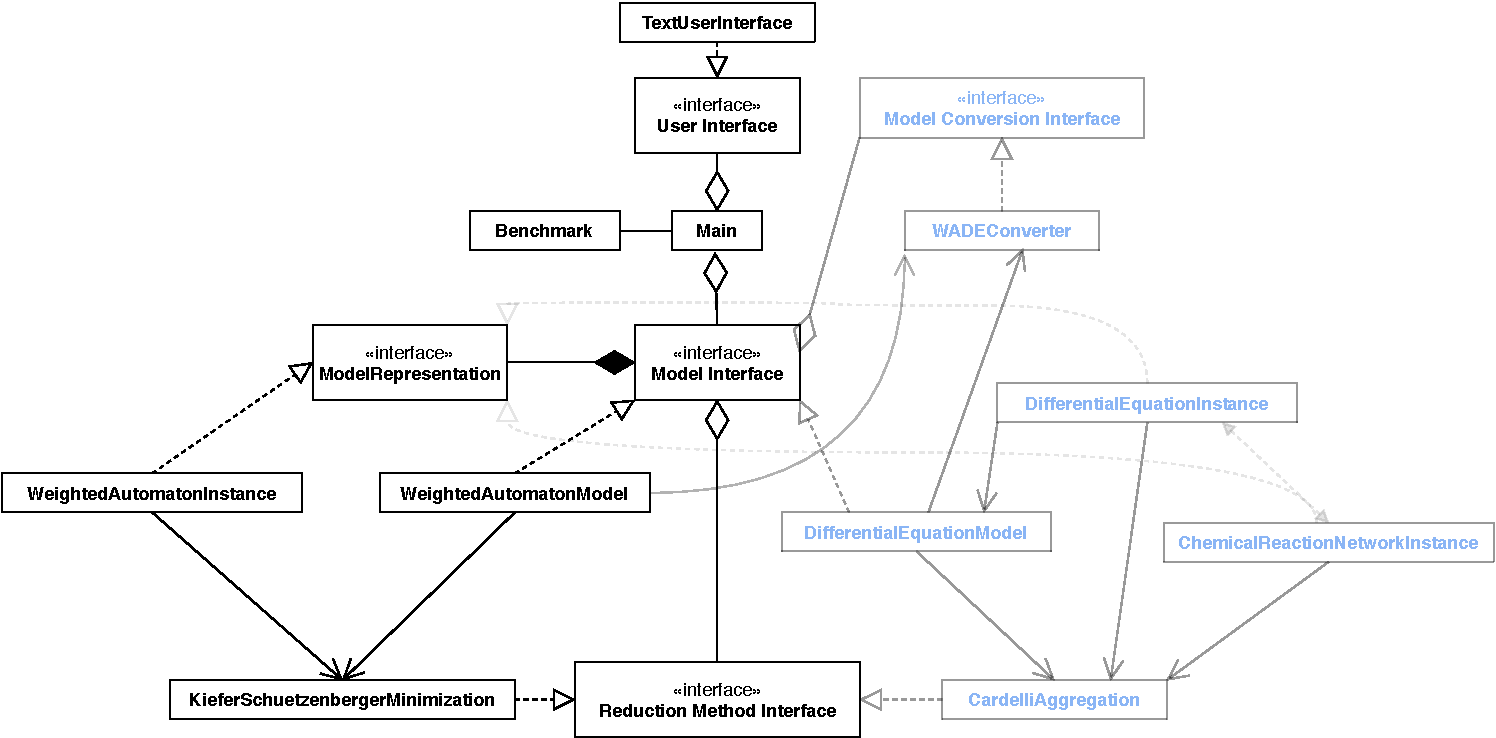
\includegraphics[keepaspectratio, height=0.8\textheight, width=\textwidth]{img/class_compact_wa.pdf}
        \end{center}
        \framebreak
        
        Sparse vs. Dense Matrices \\ \vspace{0.5cm}
        Templates,Concepts and Eigen Wrapper \\ \vspace{0.5cm}
        OpenMP multi-threadding pragmas \\ \vspace{0.5cm}
        further optimization possibilities \\ \vspace{0.5cm}
        Code \& Demo \\ \vspace{0.5cm}
    \end{frame}
    
    
    \begin{frame}{Up Next}
        Previously greyed out part: Ordinary Differential Equations \& Cardelli et al.~\autocite{Cardelli2017MaximalAO} \\ \vspace{0.5cm}
        What's the connection now? \alert{extremely sloppy notation ahead:} \\
        \[ \text{LTS} \leftrightarrow \text{WA} \leftrightarrow \text{PA} \leftrightarrow \text{MC} \leftrightarrow \text{Rule-based Modeling} \leftrightarrow \text{ODE} \leftrightarrow \text{DE} \]
    \end{frame}
  
    
    \begin{frame}{Bibliography}
        \printbibliography
    \end{frame}
\end{document}
